\documentclass[letterpaper,12pt]{article}
\usepackage[margin=.5in]{geometry}
\usepackage{xltxtra}
\setmainfont[Mapping=tex-text]{Liberation Serif}
\setmonofont[Scale=0.8]{Liberation Mono}
\newcommand{\var}[1]{\texttt{\$\{#1\}}}
\usepackage[colorlinks=false,pdfborder=0 0 0]{hyperref}
\usepackage{graphicx}

\title{Instalog Project Proposal}
\author{
Billy R. O'Neal III (bro4@case.edu) \\
Jacob Snyder (jrs213@case.edu)
}

\begin{document}

\maketitle



\section{Background}
Instalog is a senior project proposal by Jacob Snyder (jrs213) and Billy O�Neal
(bro4).
At a high level, Instalog is a tool designed to gather as much information from
a Windows machine as can feasibly be put into a small, readable log report. Such
tools are commonly used for remote support, particularly for removing malicious
software from people�s machines. In some respects, one might consider this a
solved problem. Several tools to accomplish this already exist, such as:
\begin{itemize}
  \item TrendMicro's Hijack This
  \item ``sUBs'''s Doesn't Do Squat (DDS)
  \item ``random/random'''s Random's System Information Tool (RSIT)
  \item ``OldTimer'''s OTL (Formerly OTListIt)
  \item ``OldTimer'''s OTS and OTA pair (Formerly OTScanIt and OTAnalyzeIt)
\end{itemize}

\noindent{} However, these tools all have serious problems, which we believe we
can fix in a similar tool:
\begin{itemize}
  \item Incorrect handling of some types of user data
  \item Ambiguous report formats that easily lead to machine destroying mistakes
  \item No published specifications
  \item No, or extremely buggy/complicated user interfaces
  \item Slow log generation
  \item No open source implementations available
  \item Outstanding bugs that their authors are unwilling or unable to fix
  \item No scriptability
  \item Lack of 64-bit support
\end{itemize}



\section{Introduction}
We can't entirely fault these other tools for having deficiencies.  Tools of
this variety are quite complex due to the many different loading points that
these tools report.  We think that by creating a tool that is open-source, it
will be easier for the community and us to address bugs.  This would be the
first tool of its nature that is open-source.

Moreover, the similar tools available are designed to help the remote
administrator or the local administrator, but make design compromises that make
operating on a system cumbersome for one or the other. We believe we can fix
these problems and produce a tool that is more safe, more scalable, more
performant, and easier to use than similar tools currently available.
We have conducted surveys of forums which commonly use similar logging tools,
and have support from their staff for beta testing. If we have a user base
similar to our ``spiritual predecessor'' DDS, that will be tens of thousands of
computers, running hundreds of thousands of pieces of malware, per month.



\section{Intended Users}
Instalog is designed with three types of target users in mind. These ``user
classes'' are listed in the following sections.

\subsection{Home Users}
For a typical home user, Instalog must not display a complicated interface, and
must make it relatively difficult to misstep and take a wrong action. Few
options need be presented, such as the ability to generate a default report and
the ability to take a given script and run it on a target machine. Complicated
features such as analysis must not be displayed; though they may appear as
options that are, by default, deselected.

\subsection{Administrators}
Administrators are similar to home users in that they are physically working at
a computer being examined, but they are different in that they have the intent of
repairing their own computer or the computer of a client. They wish to see
analysis features and more possible options. Instalog must provide a means for
Administrators to use it's analysis features without manual saving and reloading
of log files.

\subsection{Forum Experts}
Forum Experts help typical end users repair their machines remotely over
self-help forums such as BleepingComputer.com or GeeksToGo.com.
These users work remotely, and likely will never see a given target
machine.
Instalog must produce log formats that are human readable in the vast majority
of cases, but which can be passed through common forum software such as Invision
Power Board, phpBB, or vBulletin without destruction of information.
Unfortunately, this makes common data exchange formats such as JSON and XML
unsuitable. 

Moreover, as obtaining additional information from a machine may
have lead times of several days, Instalog's report must be unambiguous; that is,
no two possible system configurations may produce the same output. Experts can
also benefit from log analysis features. Finally, Experts need to be able to
write simple, human readable scripts to perform actions to fix a user's machine
remotely.



\section{Application Requirements}
The requirements for this tool are rather lengthy.  In fact, just listing them
requires a considerable amount of space.  Therefore, it is beyond the scope of
this document to list the full specification for any of these.  For more
information on any given requirement, please refer to the longer specification
document.  
\subsection{Logging Requirements}
One of the main features of this tool is the logging capability.  The log will
be separated into multiple ``sections,'' where each section has similar
information grouped under it.  There will be a default script of actions that is
provided with the tool that will be performed as the first part of this tool.   
There will also be additional script actions that a script can specify to gather
more targeted information about a system.
\subsubsection{Default Log Sections}
Below are the default log sections that should be presented after a default scan
has been run.
\begin{enumerate}
    \item Header
    \item Running Processes
    \item Machine PsuedoHJT Report
    \item $n$ User PseudoHJT Reports (One for each loaded user registry on the
    system)
    \item Mozilla Firefox (if Mozilla Firefox is installed)
    \item Google Chrome (if Google Chrome is installed)
    \item ``Interesting'' files present on the filesystem based on date, time,
    location, etc.
    \item Event Viewer (if any relevant events need be reported)
    \item Machine Specifications
    \item Restore Points
    \item Installed Programs
    \item Footer
\end{enumerate}
\subsubsection{Additional Log Sections}
These log sections are not included in the default scan, but can be run
optionally through a custom script.
\begin{enumerate}
\item DNS Check
	\item Directory 
	\item VirusTotal 
	\item MRC Upload
	\item Process Kill
	\item File Quarentine
	\item Security Center
	\item Registry 32 Bit
	\item Registry 64 Bit
\end{enumerate}

\subsection{Fix Script Requirements}
A fix script is a textual representation of the actions that should be taken to
clean up a system.  Most of the log sections listed in the previous section will
have fix actions associated with them.  Again, the specifics about this are too
detailed to include in a document of this scope, but will be explained in full
in the specification document.

\subsection{Graphical User Interface Requirements}
The graphical user interface will be the only method for interfacing with this
tool.  The interface is designed such that it will enable all three of the user
classes described in the ``Intended Users'' section to go through their
appropriate workflows.  As such, the GUI must bridge the gap between being
simple enough for home users to use yet complicated enough for power users to
build complex fix scripts.  This balance is achieved by splitting the GUI up
into several screens for completing various parts of the workflow.

Like the other sections, enumerating all of the requirements and specifications
of this would be beyond the scope of this document.  This being said, the GUI
should include the following screens:
\begin{enumerate}
  \item Main screen
  \item Running screen
  \item Run completed screen
  \item Analysis screen
  \item Analysis complete screen
  \item Finished screen
\end{enumerate}
This screens will be connected in the manner described in Figure 1.

\begin{figure}[h]
  	\centering
	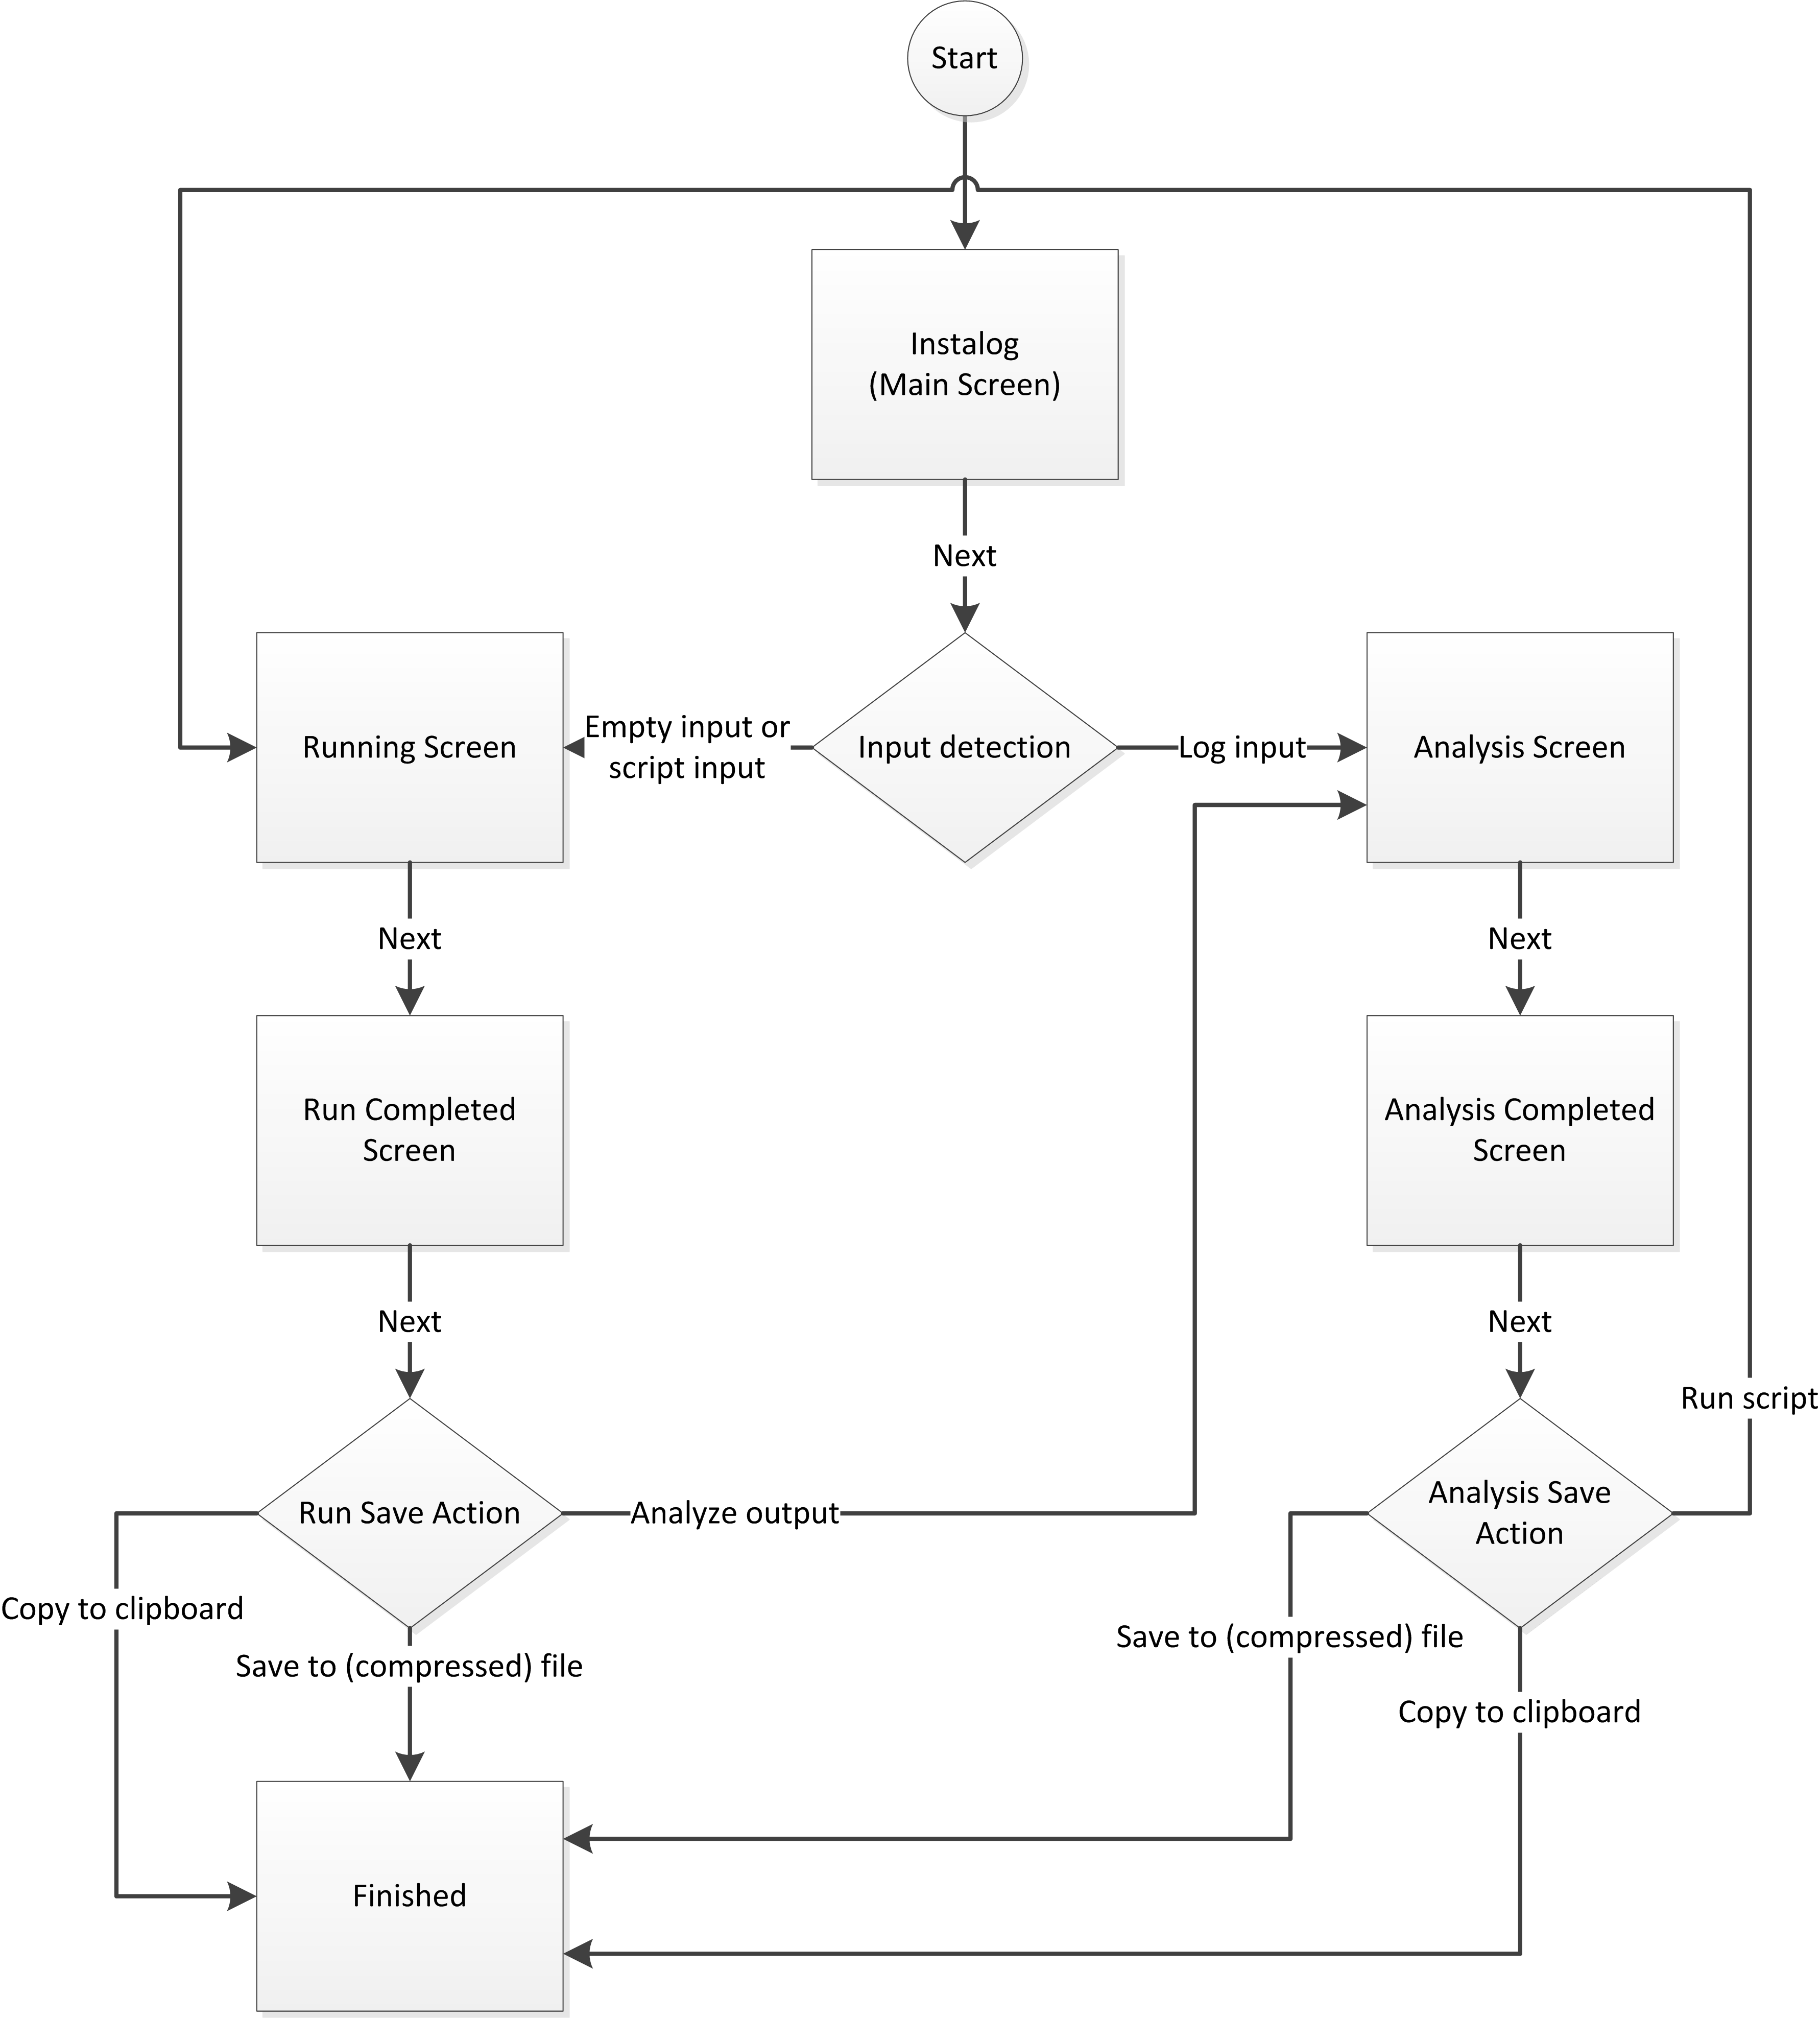
\includegraphics[scale=.5]{GUI_Flowchart.png}
  	\caption{GUI Flowchart}
  	\label{fig:gui_main}
\end{figure}

\subsection{Non-functional Requirements}
\subsubsection{Supported Operating Systems}
Instalog will support all Microsoft Windows NT variants released later than
Windows 2000 for x86 and x64 based computers.  Specifically, this tool shall
support:
\begin{itemize}
  \item Windows 2000 (x86, SP4 only)
  \item Windows XP (x86 and x64, RTM, SP1, SP2 and SP3 (on x85 machines))
  \item Windows Vista (x86 and x64, RTM, SP1, and SP2)
  \item Windows 7 (x86 and x64, RTM and SP1)
  \item Windows Server 2003 (x86 and x64, RTM, SP1, SP2)
  \item Windows Server 2003 R2 (x86 and x64, RTM, SP1, and SP2)
  \item Windows Server 2008 (x86 and x64, RTM, SP1, and SP2)
  \item Windows Server 2008 R2 (x64, RTM, and SP1)
\end{itemize}



\section{Management Plan}
\subsection{Schedule}
We will follow the schedule below for developing this tool.  This tool is
difficult to describe in a typical Gantt chart because there isn't much
interdependency between the portions of this tool.  Therefore, they could be
completed in any order.  The order provided below is a loose representation of
the order in which the project will be approached.  However, this is subject to
change.  
\begin{description}
\item[February 12] Initial draft of the specification finalized
\item[February 19] Initial draft design document finalized
\item[March 4] Logging and script actions implemented
\item[March 25] GUI implemented
\item[April 22] Testing on target systems and field testing conducted
\end{description}
\subsection{Methodology}
We will develop the logging and script actions by using a pair-programming
approach, where one team member writes the actual code and one team member
writes the tests for it.  We will then diverge and approach the GUI in a divide
and conquer method, which each team member working on disjoint portions to
finish the GUI in the short time scale allotted for it.  We will also split up
the testing for various targeted platforms.  We will create Virtual Machines of
each targeted operating system to ensure the tool runs on each system.


\end{document}
